\documentclass[12pt]{article}
\usepackage{f1000_styles}
\usepackage[numbers]{natbib}
\usepackage{hyperref}
\hypersetup{colorlinks=false, pdfborderstyle={/S/U/W 1}, pdfborder=0 0 1}
\usepackage{url}
\usepackage{setspace}

\usepackage{booktabs}
\usepackage{doi} % turn DOIs into links

\usepackage{academicons} % for ORCID icon, via https://tex.stackexchange.com/a/534476/212961
\definecolor{idcolor}{HTML}{A6CE39}
\newcommand{\orcid}[1]{\href{https://orcid.org/#1}{\color{idcolor}\aiOrcid}}

\newcommand{\email}[1]{\href{mailto:#1}{#1}}

\newcommand{\rev}[1]{#1}
%\newcommand{\rev}[1]{\textit{#1}}
%\newcommand{\rev}[1]{\textcolor{blue}{#1}}

\usepackage{fontawesome}
\newcommand{\github}[1]{\href{https://github.com/#1}{\faGithub}}
\newcommand{\twitter}[1]{\href{https://twitter.com/#1}{\faTwitter}}

\onehalfspacing
 
\begin{document}
\title{CODECHECK: an Open Science initiative for the independent
  execution of computations underlying research articles during peer
  review to  improve reproducibility}
\author[1,$\ast$]{Daniel~N\"{u}st \orcid{0000-0002-0024-5046}}
\author[2,$\ast$]{Stephen~J~Eglen \orcid{0000-0001-8607-8025}}
\affil[1]{Institute for Geoinformatics, University of M\"unster, Germany; \email{daniel.nuest@uni-muenster.de}}
\affil[2]{Department of Applied Mathematics and Theoretical Physics, University of Cambridge, UK; \email{sje30@cam.ac.uk}}
\affil[$\ast$]{Corresponding authors}
\maketitle

\begin{abstract}
 The traditional scientific paper falls short of effectively communicating computational research.  To help improve this situation, we propose a system by which the computational workflows underlying research articles are checked. The CODECHECK system uses open infrastructure and tools and can be integrated into review and publication processes in multiple ways. We describe these integrations along multiple dimensions (importance, who, openness, when). In collaboration with academic publishers and conferences, we demonstrate CODECHECK with 25 reproductions of diverse scientific publications. These CODECHECKs show that asking for reproducible workflows during a collaborative review can effectively improve executability. While CODECHECK has clear limitations, it may represent a building block in Open Science and publishing ecosystems for improving the reproducibility, appreciation, and, potentially, the quality of non-textual research artefacts. The CODECHECK website can be accessed here: \url{https://codecheck.org.uk/}.
\end{abstract}

\subsection*{Abbreviations}

ACM: Association for Computing Machinery; 
ECRs: Early Career Researchers;
RCR: Replicated Computational Results;
TOMS: Transactions on Mathematical Software.
\clearpage

\section*{Introduction}\label{introduction}

Many areas of scientific research use computations to simulate or
analyse their data. These complex computations are difficult to
explain coherently in a paper \citep{marwick_how_2015}.  To complement
the traditional route of sharing research by writing papers, there is
a growing demand to share the underlying artefacts, notably code and
datasets, so that others can inspect, reproduce or expand that work
(see Figure~\ref{fig:inverse}).  Early proponents of this initiative
were Buckheit and Donoho
\cite{buckheit_wavelab_1995,claerbout_electronic_1992}, who noted:
\emph{``An article about computational science in a scientific
  publication is \text{not} the scholarship itself, it is merely
  \textbf{advertising} of the scholarship. The actual scholarship is
  the complete software development environment and the complete set
  of instructions which generated the figures.''}

If researchers start sharing more artefacts, how might these artefacts
be examined to ensure that they do what they claim?  For example,
although scientific journals now require a data sharing statement that
outlines what data the authors have (or will) share, journals
implement this differently.  On one hand, journals have
been created to accept ``data papers''
(e.g.,~\href{https://www.nature.com/sdata/}{\emph{Scientific~Data}},
\href{https://essd.copernicus.org/}{\emph{Earth System Science Data}},
\href{https://rmets.onlinelibrary.wiley.com/journal/20496060}{\emph{Geoscience
    Data Journal}}, \href{https://bdj.pensoft.net/}{\emph{Biodiversity
    Data Journal}},
\href{https://openpsychologydata.metajnl.com/}{\emph{Journal of Open
    Psychology Data}}, \href{https://odjar.org/}{\emph{Open Data
    Journal for Agricultural Research}},
\href{https://openhealthdata.metajnl.com}{\emph{Journal of Open Health
    Data}}); these journals have established rigorous procedures by
which data are validated according to standards in each field.  On
the other hand, many journals still allow authors to
state ``Data available upon reasonable request''.  Authors, while
possibly well intentioned at the time of writing the article, often
cannot provide data when requested as data disappears over time
\cite{Vines2014-hf}.

Given that data are not routinely shared, what hope might there be for
sharing computer programs?  Both data and software are required to
validate a computational analysis; data can be seen as inert whereas
code requires an environment to be run in.  This makes software harder
to share.  Our experience is that researchers offer several reasons
for why code is not shared, e.g.,~``there is no documentation'', ``I
cannot maintain it'', or ``I do not want to give away my code to
competitors''.  Our view is that sharing code, wherever possible, is
good for the community and the individual
\cite{Barnes2010-iv,markowetz_five_2015}.  Having code and data openly
available, and archived, provides a valuable resource for others to
learn from, even if the code is broken or lacks documentation.
However, with a little effort, we believe that if an independent
person can re-run the programs, this is worth documenting and that
this reduces the barrier to evaluating non-text research materials.
Just as data journals' validations of data and all journals' peer
review provides a ``baseline reassurance'', i.e.,~that a paper has
been checked by someone with an understanding of the topic
\cite{fyfe_mission_2019}, the same baseline could be provided for the
\rev{computational} workflow underlying a paper.  With this in mind, we have developed a
set of principles and an example \rev{CODECHECK} workflow that provides a pragmatic
way of checking that a paper's code works, i.e., it is reproducible
following the Claerbout/Donoho/Peng terminology
\cite{barba_terminologies_2018}.

Here we offer a thorough description of a process and its variations
to integrate a much-needed evaluation of computational reproducibility
into peer review, and we demonstrate its feasibility by means of 25
reproductions across scientific disciplines.  We call this system
CODECHECK.

\begin{figure}
% emojis: https://github.com/googlefonts/noto-emoji
% cross mark: u274c
% check mark: u2714
  \centering
  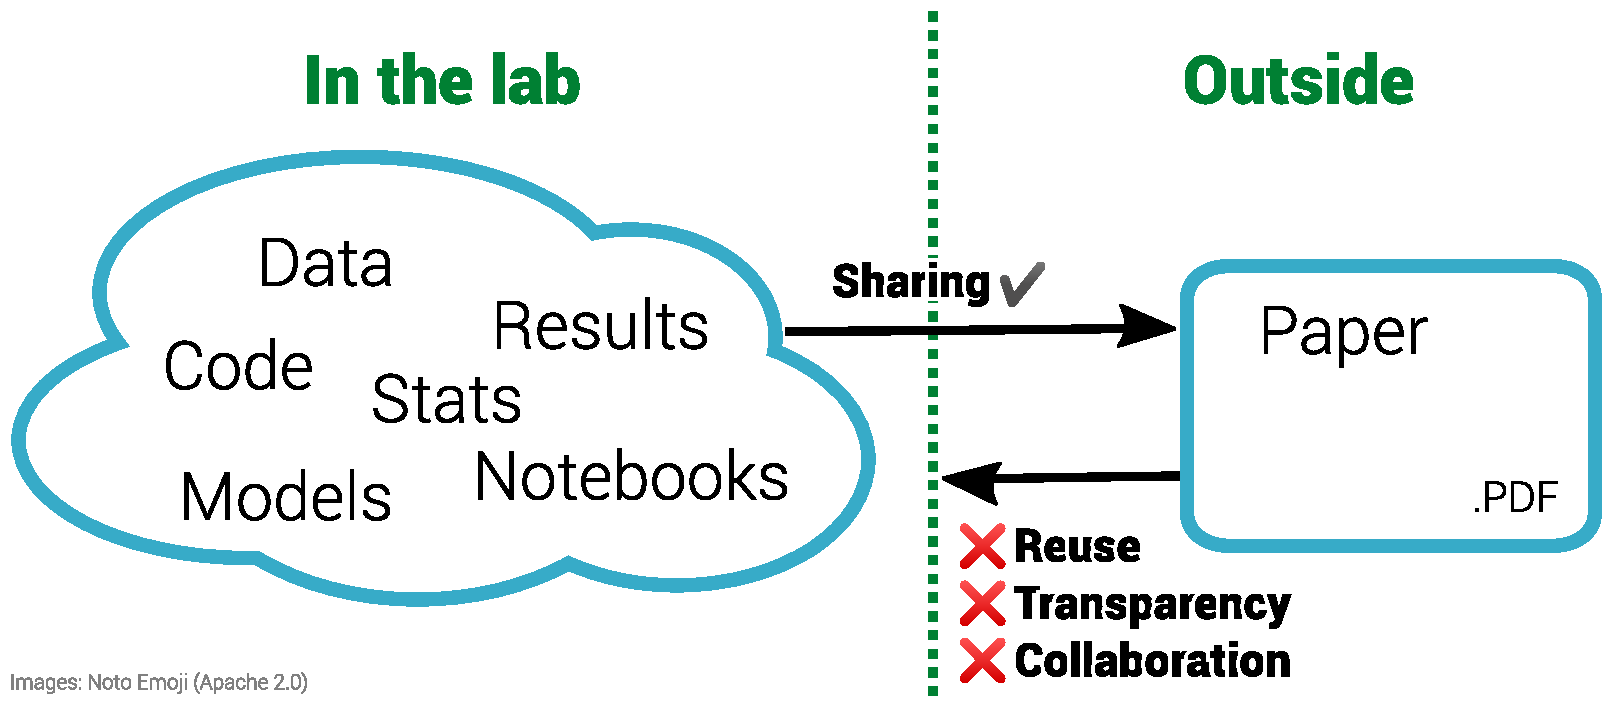
\includegraphics[width=0.7\textwidth]{figs/rr.pdf}
  \caption{The inverse problem in reproducible research. The left
  half of the diagram shows a diverse range of materials used
  within a laboratory. These materials are often then
  condensed for sharing with the outside world via the
  research paper, a static PDF document. Working backwards from the
  PDF to the underlying materials is impossible. This prohibits reuse
  and is not only non-transparent for a specific paper but is also 
  ineffective for science as a whole. By sharing the
  materials on the left, others outside the lab can enhance this work.}
  \label{fig:inverse}
\end{figure}

\section*{What is a CODECHECK?}\label{what-is-a-codecheck}

\subsection*{\rev{CODECHECK w}orkflow and people}\label{workflow-people}

CODECHECK is best demonstrated by way of our example workflow, and later
we expand on the underlying principles. The \rev{CODECHECK} workflow involves three
groups of people:
(1) the \textbf{author} of a paper providing the code to be checked,
(2) the \textbf{publisher} of a journal interested in publishing the author's paper, and
(3) the \textbf{codechecker}, who checks that the author's code works.
The six-step \rev{CODECHECK} workflow we have refined is shown in
Figure~\ref{fig:workflow}.  In this article, we also refer to a
\textbf{peer-reviewer} who is independent of this process, and
performs the traditional academic review of the content of an article.

\begin{figure}
% original figure source: https://docs.google.com/drawings/d/1tGOZFNZle-oE1Ynw_tLZFmNcv3wgxD0HPs5bXzDOrng/edit
% emojis: https://github.com/googlefonts/noto-emoji and https://github.com/twitter/twemoji
% emoji codes:
% book stack: 1f4da
% package: 1f4e6
% file drawer: 1f5c4
% disk: 1f4be
% document: 1f4c4
% phd: 1f393
% detective: u1f575
% laptop: 1f4bb
% folder: 1f4c1 1f4c2
% receipt: 1f9fe
  \centering
      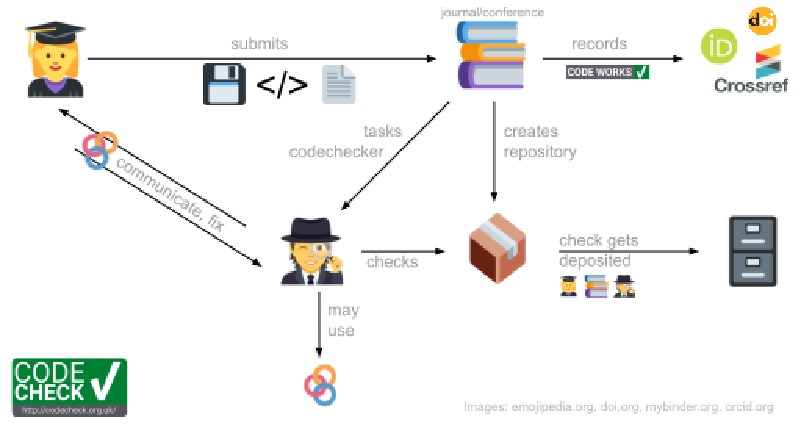
\includegraphics[width=\textwidth]{figs/codecheck_overview.pdf}
      \caption{The CODECHECK example \rev{workflow} implementation.
        Codecheckers act as detectives: They investigate and record,
        but do not fix issues.  Numbers in bold refer to steps
        outlined in the text.}
  \label{fig:workflow}
\end{figure}

\textbf{Step 1:} The author submits their manuscript along with the
code and data to the publisher.  The code and data need not be openly
available at this point.  However, in many cases the code and data may
be published on a code hosting platform, such as GitHub or
GitLab. Ideally, the author is expecting the CODECHECK and prepares
for it, e.g.,~by asking a colleague to attempt a reproduction, and
providing a set of instructions on how to re-run the \rev{computational} workflow.

\textbf{Step 2:} The publisher finds a codechecker to check the
code. This is analogous to the publisher finding one or more
peer-reviewers to evaluate the paper, except we suggest that the
codechecker and the author talk directly to each other.

\textbf{Step 3:} The codechecker runs the code, based on instructions
provided by the author. They check if some or all of the results from
the paper can be reproduced. If there are any problems running the
code, the codechecker asks the author for help, updates, or further
documentation.  The burden to provide reproducible material lies with
the author.  The codechecker then tries to run the code again.  This
process iterates until either the codechecker is successful, or the
codechecker concludes the \rev{paper's} workflow is not reproducible.  As part of
this process, the codechecker could work entirely locally, relying on
their own computing resources, or in the cloud, e.g.,~using the open
MyBinder infrastructure \cite{jupyter_binder_2018} or alternatives,
some of which are more tailored to scientific publications while
others offer commercial options for, e.g.,~publishers
(cf. \cite{konkol_publishing_2020}).  A cloud-based infrastructure
allows for the codechecker and author to collaboratively improve the
code and enforces a complete definition of the computing environment;
but, unless secure infrastructure is provided, e.g.,~by the publisher,
this requires the code and data to be published openly online.  Note
that the task of the codechecker is to check only the ``mechanics'' of the
\rev{computational} workflow.  In the context of
mathematics, Stodden et~al. \cite{stodden_setting_2013} distinguish
between \emph{verification} and \emph{validation}; following their
definition, a CODECHECK ensures verification
%\footnote{Note this is a different use from that referred to as the \emph{Verification Reports} article type in the journal \emph{Cortex} \cite{chambers_verification_2020}.},
of computational results, i.e.,~checking that code generates the
output it claims to create, but not a validation, i.e.,~checking that
the code implements the right algorithm to solve the specific research
problem.  Nevertheless, simply attempting to reproduce an output may
highlight a submission's shortcomings in meeting a journal's
requirements (cf.~\cite{christian_journal_2020}) and may effectively
increase transparency, thereby improving practices
(cf.~\cite{nosek_scientific_2012}) even if the check does not go into
every detail.

\textbf{Step 4:} The codechecker writes a certificate stating how the
code was run and includes a copy of outputs (figures or tables) that
were independently generated.  The certificate may include
recommendations on how to improve the material.  The free text in the
certificate can describe exactly what was checked, because each
\rev{computational} workflow is unique.  Since no specific tool or platform is required,
such that no authors are excluded, it is futile for the
codechecker to use automation or fixed checklists.

\textbf{Step 5:} The certificate and auxiliary files created during
the check, e.g.,~a specification of a computing environment, data
subsets or helper scripts, and the original code and data get
deposited in an open archive unless restrictions (data size, license
or sensitivity) apply.  Currently, codecheckers deposit the material
on Zenodo themselves, but a publisher may complete this step after
integrating CODECHECK into its review process.  A badge or other
visual aid may be added to the deposit and the paper and link to the
certificate.  Although a badge simplifies the CODECHECK into a binary
value and risks introducing confusion regarding the extent of the
check, a badge provides recognition value and acknowledges the
completed CODECHECK.  The badge and the actual check are incentives
for undertaking the effort needed to provide a reproducible workflow.

\textbf{Step 6:} The publisher can, depending on the timing, provide
the certificate to peer-reviewers or editors or publish it and link
between certificate, paper, and any repositories. Currently, the
codechecker creates these connections on Zenodo. They appear as links
with a relationship type on the Zenodo landing page for a certificate,
e.g., the ``related identifiers'' and ``alternate identifiers'' of
certificate \texttt{2020-025} \cite{cert-2020-025}.  The publisher
also credits the codechecker's work by depositing the activity
in scholarly profiles, such as ORCID (see peer review contributions in
\href{https://support.orcid.org/hc/en-us/articles/360006971333-Peer-Review}{ORCID records}).
The publisher also ensures proper publication metadata, e.g.,~links
from the certificate repository to the published paper or the original
code repository.

\subsection*{Variations}\label{variations}

\subsubsection*{Dimensions of CODECHECK workflows}\label{dimensions-of-workflows}

Our workflow is just one of many possibilities of a CODECHECK
workflow.  Here we consider several dimensions in a space of possible
CODECHECK workflows(Figure~\ref{fig:dimensions}).  These aspects touch
on timing, responsibilities, and transparency.

\begin{figure}
% original figure source: https://docs.google.com/drawings/d/1q2EdW3Ad-IpcD-CeoR1eIFMJW2fF6OVmDhCtCUmLO1k/edit
  \centering
      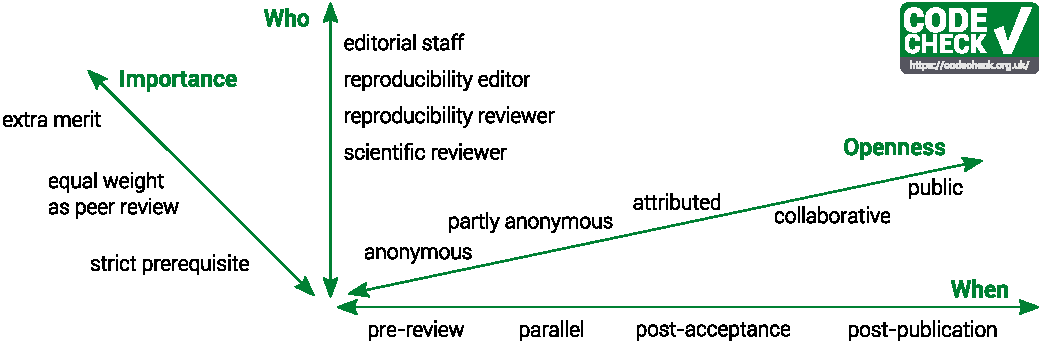
\includegraphics[width=0.8\textwidth]{figs/codecheck_dimensions.pdf}
  \caption{The dimensions of implementing a CODECHECK \rev{workflow}.}
  \label{fig:dimensions}
\end{figure}

\subsubsection*{When to do a CODECHECK and with what importance?}
\label{when-to-do-a-codecheck}

The time at which a CODECHECK is done and its ascribed importance are
closely connected, so we describe the dimensions \emph{When} and
\emph{Importance} together.  The earlier a CODECHECK happens in the
publishing process, the more it can affect editorial decisions: Is a
paper published, sent back for revisions, or rejected?  Even earlier
checks, i.e.,~a CODECHECK of a preprint, may help to improve the
\rev{computational} workflow itself, even before a publisher is involved.  As such,
codechecking papers could be part of a preprint server's policy or
initiated by interested authors.

Publishers could introduce a CODECHECK as a \textbf{strict prerequisite}.
As this can reduce the workload of reviewers, such a check should occur early in the review process.
Yet, the later in the review process the check happens, the easier is
it to allow bidirectional communication between the author and
codechecker, e.g., because the author might already be notified of the
paper's acceptance and may be more willing to share materials online closer to the paper's publication date.
A \textbf{pre-review} CODECHECK means editors would send a submission
for peer review only if it passes the check, or include the certificate in the submission package provided to peer-reviewers.
Peer-reviewers may then judge the relevance of the computations for the results of the work.

A CODECHECK may also be conducted in \textbf{parallel} to the academic
peer review.  This puts less burden on the turnaround time for the
CODECHECK, yet it only makes the outcomes available during the final
consideration by the handling editor.  The check could also be
assigned after suggestion by a reviewer, which would remove the need
for submissions to undergo a pre-review screening.  However,
soliciting such a ``specialist review'' is much less desirable than
having a regular CODECHECK, thus avoiding the situation in which some
submissions get special treatment. In both cases, the editor's
decision could be based both on CODECHECK and peer-review reports.

A \textbf{post-acceptance} CODECHECK would have the smallest impact on
editorial decisions and may simply provide \textbf{extra merit} on top
of the submission's acceptance.  This is the least impactful solution
in which all material is still evaluated and the results of the check
are properly acknowledged, because the check can be completed before
publication of the paper.  The GIScience checks (see
below) falls into this category: by displaying a badge on the volume
and article landing pages, the AGILE conference highlights articles
whose reproducibility was confirmed.  Similarly, in
collaborations with journals, some GIScience articles were
checked whilst authors worked on revisions.

A CODECHECK may also be conducted \textbf{post-publication}, though
this requires an update to the article and article metadata to
reference the check so that readers can find the CODECHECK.  In
general, publishers hesitate to make such revisions to published
articles.  We do not prefer this option as it has the least impact on
current publishing practices and downplays the importance
of reproducible workflows for ensuring good scientific practice.

%The timing of a CODECHECK needs connecting to typical scholarly communication process.
%While ideas exist for radically changing how researchers can share their work
% \footnote{For example Octopus, \url{https://science-octopus.org/about}, or Hypergraph, \url{https://www.libscie.org/hypergraph}.},
% % mimosa is another platform idea, but no real prototype AFAICT:
% % https://projects.invisionapp.com/share/E9Z3RKE7W3P#/screens/436978924
% % https://docs.google.com/presentation/d/1V_K8hghgnvGfEtW7TdwtowTveZyy4Qs8rMemNyHx_Dg/edit#slide=id.p
% an evolutionary approach has value, and we do not yet suggest to completely eliminating research papers as a way of sharing work.
Enhancing existing \rev{review and publication} processes with CODECHECKs allows communities to
gradually transition towards more open practices.
When integrating a CODECHECK into existing review and publication processes, the \emph{turnaround time} is crucial.
Depending on when and who conducts the check, it might be done quickly
or it might delay publication.
We found that a CODECHECK generally takes  2--5 hours, with some outliers on the higher end.
This time includes writing and publishing the certificate but excludes
actual computation time, some of which took days.
These efforts are comparable to the time needed to peer review a submission,
which aligns with the efforts some volunteer codecheckers are willing to
make.
Currently, there is considerable amount of communicating about the \rev{CODECHECK workflow}, especially regarding who publishes which document when, so that proper
cross-referencing between paper and certificate is ensured via persistent
identifiers.  When integrated into a peer review platform, this
handling of documents should become much more streamlined.

\subsubsection*{Openness, or ``Who knows who?''}\label{who-knows-who}

Anonymity is broadly discussed, especially in the push towards
open peer review as part of the Open Science movement 
(cf. \cite{ross-hellauer_guidelines_2019}).
Without taking a strong stance on this topic, our motivation 
behind CODECHECK
for higher transparency and reproducibility does indeed favour a more open 
review process.
However, anonymity can protect individuals
\cite{tennant_limitations_2020}, e.g.,~junior scientists.  
The negative effects of a signed review may be reduced if a CODECHECK is not relevant for a journal's decision to accept or reject, but that is, of course, not desirable when the goal is higher transparency and reproducibility.
Instead, CODECHECK is a technical process that should generally find fixable problems; it is not aimed at giving an opinion or identifying a faulty approach.
If passing a CODECHECK becomes mandatory, full transparency may need
revisiting as the relations between authors and codecheckers would fall under the
same social and community challenges as open peer review
(cf.~\cite{everythinghertz123}).
% previous sentence inspired by https://osf.io/9cftx/

The technical nature of the check and the challenge of providing sufficient documentation is why we see great benefits in bidirectional communication between author and codechecker.
Instead of trying to
fix problems or guess the next step, the codechecker can ask the author to 
rework the documentation or update code.
Instead of struggling to provide perfect instructions and as a result possibly not sharing any code or data, the author can make a best effort to document sufficiently.
Authors and readers can profit from a codecheckers' experience and approach, as during the check they may create useful and instructive files, e.g.,~a machine-readable computing environment specification.
While communication between author and codechecker may be anonymised via
the publisher, it most likely only helps to protect the identity of
the codechecker, because code is hard to anonymise.
Therefore, the most effective and desirable situation for the
stakeholders is to hold a open and collaborative CODECHECK.
The contributions by the codechecker may even be integrated into
the code of the \rev{paper's} workflow and be acknowledged as code commits. This way, 
proper credit can be given within the research software development community.


\subsubsection*{Who does the CODECHECK?}\label{who-does-the-codecheck}

Just as with peer-reviewers, a potential codechecker should have the
right skills and availability to do the work.  Ideally, the
codechecker has a matching code \emph{and} domain expertise to the
paper, although a well-documented \rev{analysis} should be executable by any
computationally-competent person. Naturally, the more
prerequisite knowledge the codechecker has, the quicker they can
understand the goals and mechanics of an analysis.  From our
experiences, the priority should be given to matching technical
expertise first, as lacking knowledge in setting up a computing
environment with a particular language or tool is much more of a
problem than assessing the outcome, e.g.,~comparing created figures
with the original, without an in-depth understanding of the domain.
The depth of the check will mostly be driven by the time required and
expertise of the checker, though in general, we expect a CODECHECK 
to consider reproducibility of the results above performance of the code.


Codecheckers could be drawn from a regular pool of
\textbf{peer-reviewers}, or from a special group of
\textbf{reproducibility reviewers} via specific roles such as
\textbf{reproducibility editors}, or \textbf{editorial staff} with a
publisher.  One codechecker is sufficient to verify the \rev{paper's} workflow since
it is mostly a factual process.  Code usually harbours systematic and
repeatable mistakes and is thereby more reliable and auditable than
processes controlled by humans \cite{tibav:42484}, e.g.,~in a
laboratory.  If however publication of the paper depends on the
CODECHECK, a second opinion may be required.

We also see a great opportunity to involve \emph{early-career
  researchers} (ECRs) as codecheckers.  ECRs arguably have a high
interest in learning about new tools and technologies, to build up
their own expertise.  CODECHECK offers a way for ECRs to gain insights
into new research and highlight the importance of reproduction.
\emph{ReScience X}, a journal devoted to reproduction and replication
experiments \cite{roesch_new_2020}, shares an interest in this
combination.  ECRs are also often familiar with new technologies, thus
also making them likely to author CODECHECK-ready manuscripts.  A
supporting data point for ECRs as early adopters is that they are
responsible for 77\% of 141 registered reports that were submitted
\cite{chambers_registered_2019}.  As ECRs are introduced to peer
review as codecheckers, they may transition into the role of
peer-reviewer over time.  Overall, we see several opportunities
and benefits to setting up a new process for codechecking with a clear
commitment to openness and transparency, independent of the current
peer review process (see \emph{Openness} dimension).

The codechecker could be a member of \textbf{editorial staff}; this is
the most controlled but also resource-intensive option.  Such a
resource commitment would show that publishers are investing in
reproducibility, yet this commitment may be hard for small publishers.
These codecheckers could be fully integrated into the internal \rev{publication process}.
Credit for doing the codecheck is also achieved, as it is part of
their duties.  By contrast, it is useful for researchers to be
publicly credited for their reviewing activity.  A regular review
may be listed in public databases (e.g.,~ORCID, see Step~6 above,
or commercial offerings such as \href{https://publons.com/about/home/}{Publons}, and
\href{https://www.reviewercredits.com/}{ReviewerCredits});
a codechecker could be similarly listed.
% The number of scientific reviews is of course only a coarse indicator of an individual's community contribution, yet it is unclear if a regular reviewer, who conducts a regular scientific review and in addition also conducts a CODECHECK, should be credited twice.
% In this case, the published CODECHECK certificate and possibly the published peer review can clearly describe the possibly large efforts put into both.

The codechecker community has over 20 volunteers who signed up in the last
year, see \url{https://github.com/codecheckers/codecheckers/}.  Their
motivations, mentioned in the \href{https://github.com/codecheckers/codecheckers/labels/registration}{registration
information},
include: supporting reproducible research and Open Science, improve
coding skills, gaining experience in helping scientists with their
code, encouraging a sharing culture, and learning from other people's
mistakes; many are also motivated simply by curiosity.  We see
benefits to an open shared list of codecheckers across journals rather
than a private in-house group, as this may allow for better matches
regarding expertise and workload sharing.  
This community can establish CODECHECK as a viable option
for independent no-cost Open Access journals.

\section*{Core principles}\label{core-principles}

The \rev{CODECHECK} workflow and variations outlined describe our current
views on how code could be checked.  They are not immutable, but
we believe the following core principles underpin our CODECHECK
\rev{workflow}:

\textbf{1. Codecheckers record but don't investigate or fix.} \\
The codechecker follows the author's instructions to run the code. If
instructions are unclear, or if code does not run, the codechecker
tells the author. We believe that the job of the codechecker is not to
fix these problems but simply to report them to the author and await a
fix.  The level of documentation required for third parties to
reproduce a \rev{computational} workflow is hard to get right, and too often this
uncertainty leads researchers to give up and not document it at all.
The conversation with a codechecker fixes this problem.

\textbf{2. Communication between humans is key.} \\
Some code may work without any interaction, e.g. \cite{cert-2020-013},
but often there are hidden dependencies that need adjusting for a
particular system.  Allowing the codechecker to communicate directly
and openly with the author make this process as constructive as
possible; routing this conversation (possibly anonymously) through a
publisher would introduce delays and inhibit community building.

\textbf{3. Credit is given to codecheckers.} \\
The value of performing a CODECHECK is comparable to that of a peer
review, and it may require a similar amount of time. Therefore, the
codechecker's activity should be recorded, ideally in the published
paper.  The public record can be realised by publishing the
certificate in a citable form (i.e.,~with a DOI), by
listing codecheckers on the journal's website or, ideally, by
publishing the checks alongside peer review activities in public
databases.

\textbf{4. \rev{Computational} workflows must be auditable.} \\
The codechecker should have sufficient material to validate the
\rev{computational} workflow outputs submitted by the
authors. Stark~\cite{stark_before_2018} calls this
``preproducibility'' and the ICERM report \cite{stodden_setting_2013}
defines the level ``Auditable Research'' similarly.  Communities can
establish their own good practices or adapt generic concepts and
practical tools, such as publishing all building blocks of science in
a research compendium (cf.~\url{https://research-compendium.science/})
or ``repro-pack'' \cite{barba_praxis_2018}.  A completed check means
that code could be executed at least once using the provided
instructions, and, therefore, all code and data was given and could be
investigated more deeply or extended in the future.  Ideally, this is
a ``one~click'' step, but achieving this requires particular skills
and a sufficient level of documentation for third
parties. Furthermore, automation may lead to people gaming the system
or reliance on technology, which can often hide important details.
All such aspects can reduce the understandability of the material, so
we estimate our approach to codechecking, done without automation and
with open human communication, to be a simple way to ensure long-term
transparency and usefulness.  We acknowledge that others have argued
in favour of bitwise reproducibility because, in the long run, it can
\rev{help to automate checking by comparing outputs algorithmically} (e.g.,
\url{https://twitter.com/khinsen/status/1242842759733665799}), but
until \rev{such an ideal is achievable} we need CODECHECK's approach.

\textbf{5. Open by default and transitional by disposition.} \\
Unless there are strong reasons to the contrary
(e.g.,~sensitive data on human subjects), all code and data, both from
author and codechecker, will be made freely available when
the certificate is published.  Openness is not required for the paper
itself, to accommodate journals in their transition to
Open Access models.  The code and data publication should follow
community good practices.  Ultimately we may find that CODECHECK activities are
subsumed within peer review.
%% By disposition, a CODECHECK workflow should
%% be designed (a) recognising shortcomings in asserting reproducibility
%% of submissions and (b) with an understanding of the complex situation
%% that led to this. However, establishing a CODECHECK workflow should
%% mirror initiatives to improve education around reproducibility of
%% methods.  The long term goal is for a specific community to reach a
%% state where the level of verification ensured by codecheckers becomes
%% part of peer review and a regular merit of all accepted papers.

\section*{Implementation}\label{implementation}

\subsection*{Register}\label{register}

To date we have created 25 certificates (Table~\ref{tab:register}) 
falling into three broad themes: (1) classic and current
papers from computational neuroscience, (2) COVID-19 modelling
preprints, and (3) GIScience.

The first theme was an initial set of papers used to explore the
concept of CODECHECK.  The idea was to take well-known articles from a
domain of interest (Neuroscience).  Our first CODECHECK (certificate
number \texttt{2020-001}) was performed before publication on an
article for the journal \emph{GigaScience}, which visusalized the
outputs from a family of supervised classification algorithms.

The second theme was a response to the COVID-19 pandemic, selecting
papers that predicted outcomes. The checks were solicited through
community interaction or by our initiative rather than requested from
journals.  Some certificates were since acknowledged in the accepted
papers \cite{Davies2020-vj,kucharski_effectiveness_2020}. In
particular, we codechecked the well-known Imperial college model of UK
lockdown procedures from March 2020,
demonstrating that the model results were reproducible
\cite{Chawla2020-hi,cert-2020-010}.

The third theme represents co-author DN's service as a Reproducibility
Reviewer at the AGILE conference series, where the \emph{Reproducible
  AGILE} Initiative \cite{reproducible_agile} independently
established a process for reproducing \rev{computational} workflows at the AGILE
conference series \cite{nust_improving_2020}.  While using slightly
different terms and infrastructure (``reproducibility reports'' are
published on the Open Science Framework instead of certificates
on Zenodo) AGILE reproducibility reviews adhere to CODECHECK
principles.  A few checks were also completed as part of peer reviews
for GIScience journals.

\begin{table}
  \footnotesize

  \centering

  \begin{tabular}{llp{12cm}}
    \toprule
    \textbf{Certificate} & \textbf{Research area} & \textbf{Description} \\ \midrule
    \texttt{2020-001} \cite{cert-2020-001} & Machine learning & Code for benchmarking ML classification tool checked post acceptance of manuscript and before its publication in \textit{Gigascience} \cite{Piccolo2020-lo}. \\
    \texttt{2020-002}  \cite{cert-2020-002} & Neuroscience & Code written for this project checked by second project member as demonstration using paper from 1997 showing unsupervised learning from natural images \cite{Hancock1992-mp}. \\
    \texttt{2020-003}  \cite{cert-2020-003} & Neuroscience &  Code written for this project checked by second project member as demonstration using classic paper on models of associative memory \cite{Hopfield1982-mz}. \\
    \texttt{2020-004}  \cite{cert-2020-004} & Neuroscience & Code written for this project checked by second project member as demonstration using classic paper on cart-pole balancing problem \cite{Barto1983-rg}. \\
    \texttt{2020-005}  \cite{cert-2020-005} & Neuroscience & Check of independent reimplementation of spike-timing-dependent plasticity (STDP) model \cite{larisch_re_2019} conducted as demonstration for this paper. \\ % Python ANNarchy
    \texttt{2020-006}  \cite{cert-2020-006} & Neuroscience & Check of independent reimplementation of a generalized linear integrate-and-fire neural model \cite{detorakis_re_2017} conducted as demonstration for this paper. \\
    \texttt{2020-007}  \cite{cert-2020-007} & Neuroscience & Check of independent reimplementation of analysing spike patterns of neurons \cite{hathway_re_2018} conducted as demonstration for this paper. \\
    \texttt{2020-008}  \cite{cert-2020-008} & COVID-19 & Code for modelling of interventions on COVID-19 cases in the UK checked at preprint stage \cite{davies-preprint-2020} and later published \cite{Davies2020-vj}. \\
    \texttt{2020-009}  \cite{cert-2020-009} & COVID-19 & Code for analysis of effectiveness of measures to reduce transmission of SARS-CoV-2 checked as preprint \cite{kucharski-preprint-2020} and later published \cite{kucharski_effectiveness_2020}. \\ % R, check mentioned in acks, but not linked
    \texttt{2020-010}  \cite{cert-2020-010} & COVID-19 & Code for analysis of non-pharmaceutical interventions (Report 9) checked as a preprint \cite{ferguson_report_2020}. \\ % CovidSim
    \texttt{2020-011}  \cite{cert-2020-011} & COVID-19 & Code for modelling of COVID-19 spread across Europe was provided by authors and checked while paper was in press \cite{flaxman_estimating_2020}. \\
    \texttt{2020-012}  \cite{cert-2020-012} & COVID-19 & Code for modelling of COVID-19 spread across the USA was checked as preprint \cite{unwin_report_2020} and later published \cite{unwin_state-level_2020}. \\
    \texttt{2020-013}  \cite{cert-2020-013} & Neuroscience & Code for analysis of rest-activity patterns in people without con-mediated vision was checked as a preprint \cite{Spitschan2020.06.02.129502} after direct contact with the authors. \\ % MATLAB
    \texttt{2020-014}  \cite{cert-2020-014} & Neuroscience & Code for analysis of perturbation patterns of neural activity was checked after publication as part of publisher collaboration \cite{Sadeh2020}. \\ % MATLAB
    \texttt{2020-015}  \cite{cert-2020-015} & Neuroscience & Code for a neural network model for human focal seizures was checked after publication as part of publisher collaboration \cite{Liou2020}. \\ % MATLAB
    \texttt{2020-016}  \cite{cert-2020-016} & GIScience & Code for models demonstrating the Modifiable Aral Unit Problem (MAUP) in spatial data science \cite{Brunsdon2020} was checked during peer review. \\ % R
    \texttt{2020-017}  \cite{cert-2020-017} & GIScience & Code for spatial data handling, analysis, and visualisation using a variety of R packages \cite{Bivand2020} was checked after peer review before publication. \\ % R
    \texttt{2020-018}  \cite{cert-2020-018} & GIScience & AGILE conference reproducibility report using a demonstration data subset with cellular automaton for modeling dynamic phenomena \cite{Hojati2020}. \\ % R
    \texttt{2020-019}  \cite{cert-2020-019} & GIScience & AGILE conference reproducibility report with subsampled dataset for reachability analysis of suburban transportation using shared cars \cite{Illium2020}. \\
    \texttt{2020-020}  \cite{cert-2020-020} & GIScience & AGILE conference reproducibility report using a container for checking in-database windows operators for processing spatio-temporal data \cite{Werner2020}. \\ % Python + PostGIS
    \texttt{2020-021}  \cite{cert-2020-021} & GIScience & AGILE conference reproducibility report checking code for comparing supervised machine learning models for spatial nominal entity recognition \cite{Medad2020}. \\ % Python
    \texttt{2020-022}  \cite{cert-2020-022} & GIScience & AGILE conference reproducibility report checking code for visualising text analysis on intents and concepts from geo-analytic questions \cite{Xu2020}. \\ % Python
    \texttt{2020-023}  \cite{cert-2020-023} & GIScience & AGILE conference reproducibility report on analysis of spatial footprints of geo-tagged extreme weather events from social media \cite{Owuor2020}. \\
    \texttt{2020-024}  \cite{cert-2020-024} & Neuroscience & Code for multi-agent system for concept drift detection in electromyography \cite{vieira_driftage_2020} was checked during peer review. \\ % R
    \texttt{2020-025}  \cite{cert-2020-025} & GIScience & Adaptation and application of Local Indicators for Categorical Data (LICD) to archaeological data \cite{carrer_application_2021} was checked after peer review before publication. \\ % R
    \\ \bottomrule
  \end{tabular}
  \caption{Register of completed certificates as of December 2020. An interactive version
  is available at \url{http://codecheck.org.uk/register}.
  }
  \label{tab:register}
\end{table}

\subsection*{Annotated certificate and check metadata}\label{annotated-certificate}

After running the \rev{paper's} workflow, the codechecker writes a certificate
stating which outputs from the original article, i.e.,~numbers,
figures or tables, could be reproduced.  This certificate is made
openly available so that everyone can see which
elements were reproduced and what limitations or issues were found.
The certificate links to code and data used by the codechecker,
allowing others to build on the work.  The format of the certificates
evolved during the project, as we learnt to automate different
aspects of the certification.  The metadata
is stored in a machine-readable structured file in YAML, the CODECHECK
configuration file \texttt{codecheck.yml}.
The technical specification of the CODECHECK configuration file is
published at \url{https://codecheck.org.uk/spec/config/latest/}.  The
configuration file enables current and future automation of \rev{CODECHECK} workflows
and meta-analyses.

Figure~\ref{fig:cert} shows pages 1--4 (of 10) of an example
certificate to check predictions of COVID-19 spread across the USA
\cite{cert-2020-012,unwin_report_2020}.  Figure~\ref{fig:cert}A shows
the certificate number and its DOI, which points to the certificate
and any supplemental files on Zenodo.  The CODECHECK logo is added for
recognition and to denote successful reproduction.
Figure~\ref{fig:cert}B provides the key metadata extracted from
\texttt{codecheck.yml}; it names the paper that was checked (title,
DOI), the authors, the codechecker, when the check was performed, and
where code/data are available.
Figure~\ref{fig:cert}C shows a textual summary of how the CODECHECK
was performed and key findings.  Figure~\ref{fig:cert}D
(page 2 of the certificate) shows the outputs that were generated
based on the MANIFEST of output files in the CODECHECK.  It shows the
file name (Output), the description stating to which figure/table each
file should be compared in the original paper (Comment), and the file
size.  Page 3 of the certificate, Figure~\ref{fig:cert}E gives
detailed notes from the codechecker, here documenting what steps were
needed to run the code and that the code took about 17~hours to
complete. Finally, page 4 of the certificate shows the first output
generated by the CODECHECK Figure~\ref{fig:cert}F. In this case, the
figure matched figure~4 of \cite{unwin_report_2020}.  The remaining
pages of the certificate show other outputs and the computing
environment in which the certificate itself was created (not shown
here).

\begin{figure}
  \centering
  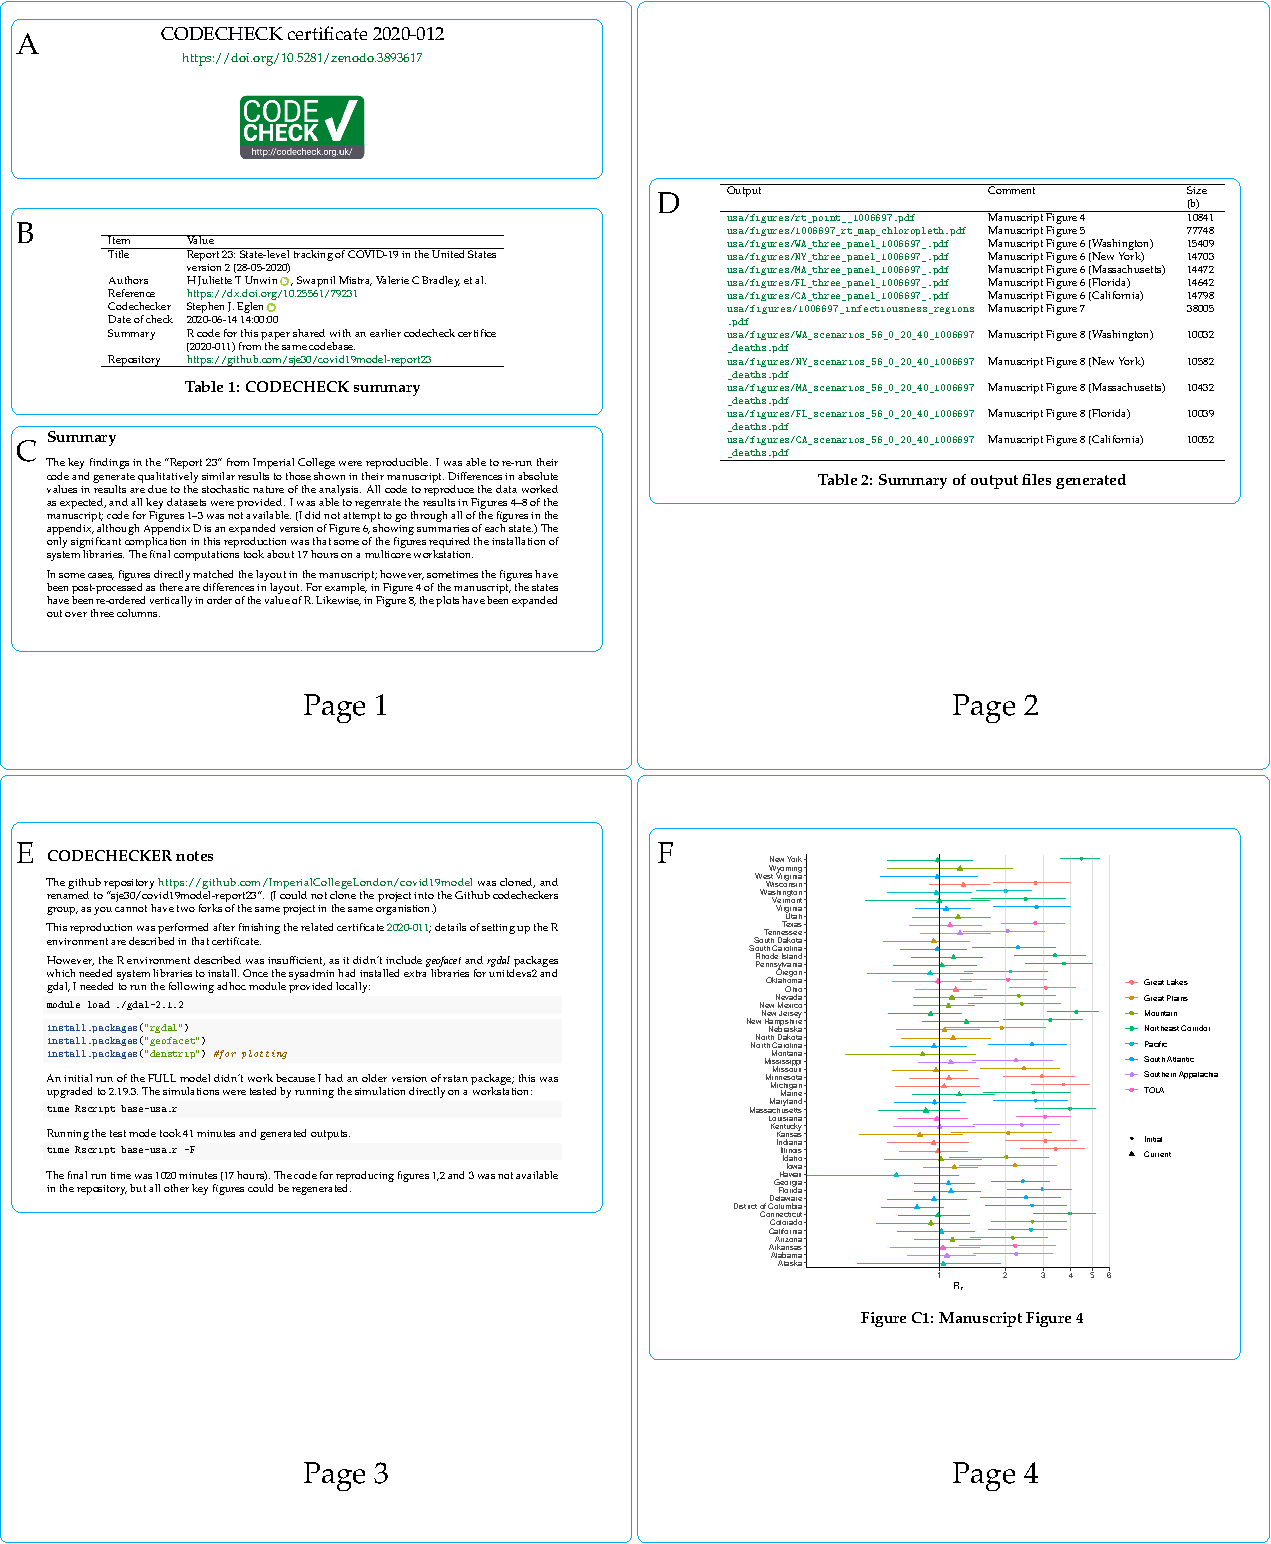
\includegraphics[width=\textwidth]{figs/annotate-cert-crop.pdf}
  \caption{Annotated certificate \texttt{2020-012} \cite{cert-2020-012} (first four pages only).}
  \label{fig:cert}
\end{figure}

\subsection*{Tools and resources}\label{tools}

We use freely available infrastructure, GitHub and Zenodo, to run our
system.  The \texttt{codecheckers} \textbf{GitHub} organisation at
\url{https://github.com/codecheckers} contains projects for managing
the project website, the codecheckers community and its discussions,
code repositories, and the main register of CODECHECKs. Both the
project website \url{https://codecheck.org.uk/} and the register at
\url{https://codecheck.org.uk/register} are hosted as GitHub pages.
The register database is a single table in CSV format that connects
the certificate identifier with the repository associated with a
CODECHECK. Each of these repositories, which currently can be hosted
on GitHub or Open Science Framework, contains the CODECHECK
metadata file \texttt{codecheck.yml}. The register further contains a
column for the type of check, e.g.,~community, journal, or conference,
and the respective GitHub issue where communications and assignments
around a specific check are organised. No information is duplicated
between the register and the metadata files. The continuous
integration infrastructure of GitHub, GitHub Actions, is used to
automate generation of the register.  \textbf{Zenodo} is our preferred open
repository for storing certificates. It mints DOIs for deposits and
ensures long-term availability of all digital artefacts related to the
project. The CODECHECK community on Zenodo is available at
\url{https://zenodo.org/communities/codecheck/}. It holds
certificates, the regularly archived register
\cite{codecheck_register_jan2021}, and other material related to
CODECHECK.

A \textbf{custom R package}, \texttt{codecheck}, automates
repetitive tasks around authoring certificates and managing the
register. The package is published at
\url{https://github.com/codecheckers/codecheck} under MIT license
\cite{stephen_eglen_codecheckerscodecheck_2021}.
It includes scripts to deposit certificates and related
files to Zenodo using the R package \texttt{zen4R} \cite{zen4r} and
for the register update process outlined above.  Codecheckers can
ignore this package, and use their own tools for creating
and depositing the certificate.  This flexibility  accommodates
different skill sets and unforeseen technical advances or challenges.

These tools and resources demonstrate that a CODECHECK \rev{workflow} can be
managed on freely available platforms.
Automation of some aspects may improve turnaround time. Our main
resource requirements are the \textbf{humans} needed for managing the
project and processes and the codecheckers.  All contributions
currently rely on (partly grant-based) public funding and
volunteering.

\section*{Related work}\label{related-work}

The journal \emph{ACM Transactions on Mathematical Software (TOMS)}
recently established a ``Replicated Computational Results'' (RCR)
review process \cite{heroux_editorial_2015}, where ``replicable'' is
the same as our use of ``reproducible''.  Fifteen RCR Reports have
been published so far (search on \url{https://search.crossref.org/}
with the term \texttt{"Replicated Computations Results (RCR) Report"}
on 2020-12-10).
% 15: https://academic.microsoft.com/search?q=Replicated%20Computations%20Results%20%22(RCR)%20Report%22&f=&orderBy=0&skip=10&take=10
and the process is being extended extended to the ACM journal
\emph{Transactions on Modeling and Computer Simulation}.
%% (cf. \url{https://dl.acm.org/journal/tomacs/author-guidelines}).
The TOMS RCR follows CODECHECK principles 1-4, although our work was
independently developed of theirs.  The TOMS editorial
\cite{heroux_editorial_2015} shares similar concerns about selection
of reviewers, as we discussed above. Unlike existing CODECHECK
certificates, the RCR reports undergo editorial review.  Publication
of the RCR report recognises the efforts of the reproducing person,
while the potential for this motive to be a conflict of interest is
acknowledged.  TOMS also recognises reviewer activity in a partnership
with Publons (see
\url{https://authors.acm.org/author-services/publons}).  \rev{As well
  as this, ACM provides several badges to indicate what kind of artifact review or reproduction a paper submitted to an ACM journal completed (\url{https://www.acm.org/publications/policies/artifact-review-and-badging-current}), but does not provide nor require a specific review process. In principle, these badges could be awarded by a codechecker, too, though the different levels and even partial replacement of artifacts required  to achieve a \emph{Results Reproduced} go beyond a CODECHECK's scope. A completed check certainly warrants the ACM badge \emph{Artifacts Evaluated - Functional} and possibly \emph{Artifacts Evaluated - Reusable} and likely \emph{Artifacts Available}, depending on additional requirements by implementing journals. However, we do not require codecheckers to evaluate code quality or ensuring proper archival of artifacts though, in our experience, they are likely to encounter or comment on these topics.}
This activity in the ACM journals can be seen as one possible \rev{process}
within a CODECHECK system, and clearly shares much in spirit.
CODECHECK, however, specifically aims to give codecheckers recognition
as reviewers.  In our view, the reviewer role removes the possible
conflict of interest while keeping the public acknowledgement.
Specific to the field of mathematics, the RCR is also expected to
apply a review of the software itself if the system it runs on cannot
be evaluated by an independent party.  The TOMS RCR creators concur
with the importance of communication, expect collaboration between
author and RCR reviewers, share the considerations around reviewer
selection, and also put trust in reviewer judgement over numerical
bit-wise perfection.  A key difference is that for TOMS RCR, authors
opt-in with an \emph{RCR Review Request} and the RCR reports are
published in the TOMS journal next to the actual papers.


Several journals provide special article types for reproductions of
published papers.  \emph{Information Systems} has an invitation only
Reproducibility Section for articles describing the reproducibility 
efforts of published articles, which are co-authored by the original
authors and the reproducibility reviewer(s) (see
\url{https://www.elsevier.com/journals/information-systems/0306-4379/guide-for-authors}).
\emph{Nature Machine Intelligence} recently introduced a new type of
article, the reusability report \cite{noauthor_research_2020}.
Inspired by the detailed and nuanced submissions to a reproducibility
challenge, the reusability report focuses on the exploration of
robustness and generalizability of the original paper's claims
\cite{noauthor_research_2020}. This answers the specific community's
challenges around computational reproducibility and also values these
kinds of contributions as independent publications, which goes beyond
the goals of CODECHECK.  The journal \emph{Cortex} has a special
article type \emph{Verification Reports}, which are actually about
replication of results and are very well designed/reasoned
\cite{chambers_verification_2020}.
\rev{The \emph{Journal of Water Resources Planning and Management}'s 
policy recognises reproducible papers in a special collection and 
incentivises authors with waived or reduced fees
\cite{rosenberg_reproducible_2021}.}
In a similar vein, the CODECHECK
certificates could also be published as a special article type within
journals.  \rev{Finally, the \textit{Journal of Open Source Software}
provides its reviewers with a checklist of items to check during
review,
\url{https://joss.readthedocs.io/en/latest/review_checklist.html\#software-paper},
effectively providing a much more detailed form of check for scientific
software that could complement CODECHECKs, too.}

Going beyond individual articles, the journal
\href{https://rescience.github.io}{\emph{ReScience~C}} publishes only
replications, also requiring open code and replication by a third
party.  \rev{The journal now accepts ``Reproduction reports'' that
  describe if some code accompanying a published article can (or can
  not) reproduce the same results as shown in the article.}  ReScience~C
also relies on free infrastructure (GitHub and Zenodo).

For research with high stakes, where reproduction would be too weak and
post-publication replication possibly too late because of policy impact,
Benjamin-Chung et~al. \cite{benjamin-chung_internal_2020} propose
\emph{internal replication}.
A \rev{computational} workflow that has undergone internal
replication would likely be of high quality and relatively easy to check.
Similarly, internal CODECHECKs may be used, with the same limitations such
as group think \cite{benjamin-chung_internal_2020},
to ensure reproducibility before submission.
Such internal checks are professionalised in local reproduction services,
such as \href{https://ciser.cornell.edu/research/results-reproduction-r-squared-service/}{CISER R-squared} or \href{https://isps.yale.edu/research/data/approach}{YARD},
or in communities such as \href{https://github.com/OxfordCodeReviewNet/forum}{Oxford's code review network}.

Gavis and Donoho \cite{gavish_universal_2011} propose a new discipline
and infrastructure for reproducible computational research. Their
specific packaging format, provenance record, and cryptographic
\emph{Verifiable Result Identifier} would indeed provide excellent
reproducibility. However, the system is also complex and since its
creation in 2011 we are not aware of any publisher using it; also, the
system is not open source.  In comparison, CODECHECK is less powerful
but also much more flexible and less dependent on specific tools or
infrastructure. If data and code are deposited properly, i.e.,~very
unlikely to disappear, then the certificate's DOI is practically close
to the cryptographic identifier.

Another platform for publishing results of reproductions is
\href{https://scigen.report}{\emph{SciGen.Report}}.  It is a
community-run independent platform to foster communication on
reproducibility.  People can report on fully, partially, or
failed reproductions of articles after publication.

CODECHECK is uniquely designed to be adopted across journals or events
and to build a community of codecheckers. CODECHECK shares its
interdisciplinary nature with other community initiatives concerned
with reproducibility awareness, education, and support, such as
\href{https://reprohack.github.io/reprohack-hq/}{ReproHack},
\href{https://twitter.com/Code_Copilot}{Code Copilot}, or
\href{https://paperswithcode.com/about}{Papers with Code}.
The latter recently announced a collaboration with the preprint server
\emph{arXiv} on providing data and code supplements for machine
learning manuscripts
%\footnote{\url{https://medium.com/paperswithcode/papers-with-code-partners-with-arxiv-ecc362883167}}
and runs a reproducibility challenge.
%\footnote{\url{https://paperswithcode.com/rc2020}}.
% Papers with Code now also does more disciplines than just ML.
Likewise, different disciplines and journals provide reproducibility
checklists, e.g.,~science and engineering \cite{rosenberg_next_2020} or
GIScience \cite{nust_agile_2019}, which naturally share some aspects
while addressing particularities as well as addressing researchers
from different fields. Regarding the education and guidance for
authors, we see CODECHECK's role as referencing and linking
educational efforts and helpful material, not as creating and
maintaining such content.

\section*{Limitations}\label{limitations}

\textbf{Isn't CODECHECK what peer review should be doing already?}  On
the surface, yes, but peer reviewers are overburdened enough and
asking them to do more work around peer review is not likely to
succeed.  When an editor (Tsuyoshi Miyakawa) requested raw data from
n=41 authors before reviewing, 21 authors withdrew their manuscripts;
19 of the 20 remaining articles were rejected after peer review
\cite{miyakawa_no_2020}.  Such basic checks require effort from
editors, yet they only rely on the availability of data files and the
content of the paper.  These availability checks can be enhanced by
having more complex CODECHECKs request the code and then execute it.
This might fall within idealistic expectations of peer review, but is
rare.  Establishing a CODECHECK \rev{workflow} acknowledges that peer
reviewing practices have been unable to adapt to the challenges of
computational papers.  The concept of a CODECHECK, just as the
concepts of reproducible research and Open Science, may be
transitional by nature. If the activities described here as being part
of a CODECHECK are integrated into the publication process the
initiative will have succeeded.

\textbf{Should CODECHECK requirements be more demanding?}
CODECHECK by design does not require authors to provide (and sustain)
an eternally functional \rev{computational} workflow nor suggests a specific software
stack or practical approach.
Creating something
that anyone can reproduce \href{https://twitter.com/DougBlank/status/1135904909663068165}{has been called a fool's
errand}
and we tend to agree.  However, the package of data, code, and
documentation collaboratively created by authors and codecheckers is a
snapshot of a working analysis that greatly increases the likelihood
of a successful reproduction and the possibility that a \rev{computational} workflow can
be extended by third parties in the future, if they have
access to suitable resources and matching skill set.
\rev{The CODECHECK principles help to make very clear what a CODECHECK
badge on a paper means and also ensure a minimum standard that 
other processes or badges may not have, e.g., only superficially 
checked self-awarded badges (
\url{https://www.cambridge.org/core/journals/environmental-data-science/information/instructions-for-authors}).}

Concrete
implementations of CODECHECK workflows, especially for specific
disciplines, may reify much more helpful guidelines for authors on how
to create reproducibility packages.  Our author-friendly ``low bar''
should not stay low forever, but cultural change takes time and the
encouragement and guidance that CODECHECK, as part of the widely
accepted peer review concept, can provide may eventually allow the bar
to be raised much higher, e.g.,~with executable research
compendia \cite{nust_opening_2017}, ``Whole Tales''
\cite{brinckman_computing_2018}, or continuous analysis
\cite{beaulieu-jones_reproducibility_2017-1}.  However, considering
that missing artefacts and lack of documentation have repeatedly been
identified as key barriers to reproducibility
(e.g.,~\cite{stagge_assessing_2019,nust_improving_2020}), we would not
underestimate the power of a simple check.  For example, ModelDB
curation policies require that only one figure need be manually reproduced
\cite{mcdougal_reproducibility_2016}, but that has not limited the
usefulness nor success of the platform.

A codechecker does not fulfil the same role as a \emph{statistical
  reviewer}, as it is applied by some journals in the biomedical
domain (cf.~\cite{petrovecki_role_2009,greenwood_how_2015}).  The
statistical reviewer evaluates the appropriateness of statistical
methods \cite{greenwood_how_2015} and can support topical reviewers
if, e.g.,~complex methods or sophisticated variants of statistical
tests are applied \cite{petrovecki_role_2009}.  The codechecker may go
equally deep into the review, but only if they have the expertise and
time. We can imagine a tiered \rev{CODECHECK} workflow where a codechecker could, just
as a conventional reviewer could, recommend a detailed code review
(see next paragraph) to the editor if they come upon certain issues while
examining the work.

A codechecker does not conduct a \emph{code review}. Code reviews are
valuable to improve reproducibility and reusability, and their
proponents even believe they can improve the research
\cite{petre_code_2014}.  Code reviews, however, have quite different
structural challenges and require even more resources. That said, a
well-reviewed codebase is likely to be easier to codecheck, and the
awareness of high-quality code raised through CODECHECK may lead to
more support for code reviewing.  Initiatives and journals that
conduct software reviews independent of a specific publication or
\rev{venue} include \href{https://ropensci.org/}{ROpenSci}, \href{https://www.pyopensci.org/}{PyOpenSci}, and \href{https://joss.theoj.org}{JOSS}.  Furthermore, the codechecker's task
list is intentionally not overloaded with related issues such as
ensuring proper citation of data and software or depositing material
in suitable repositories. Nevertheless, codecheckers are free to
highlight these issues.

\textbf{How are failures during checks handled?} We do not yet have a process for denoting if a reproduction fails, as our case-studies were all successful.  In the case that a journal
adopts CODECHECK for all submissions, the question remains as what to
do if a check fails, after exhausting efforts between author and
codechecker to reproduce the \rev{computational} workflow.  A negative comment in a
CODECHECK certificate or a failed check does not necessarily mean the
paper or research is bad (cf. discussion on negative comments in
\cite{everythinghertz123}).  We doubt that publicly reporting failures
(i.e.,~the code would not run) will increase overall reproducibility,
and may prohibit authors from sharing their work, which is always more
desirable than nothing shared. Therefore, we recommend sharing interim
reproduction efforts only with the authors, even if that means that volunteer
efforts may go unnoticed if no certificate is published.  
% eLife's new model (see https://osf.io/9cftx/) will publish reports eventually, e.g.,~after preprint has been accepted elsewhere
Rosenthal et~al. \cite{Rosenthal2016b} discuss such incentives for
different actors around the implementation of reproducibility. We see
CODECHECK as one way for organisations to invest in reproducibility by
creating incentives until reproducible computations become the norm.

\textbf{Who will pay for the compute time?}  For papers that take
significant compute time (days, not minutes), it is unclear who will
pay for it. One must carefully consider the sustainability of
rerunning computations and the environmental impact large
calculations, such as training machine learning models, have.  A
pragmatic workaround is to request that authors provide a ``toy''
example, or small dataset that can be quickly analysed to demonstrate
that the \rev{paper's} workflow runs correctly.

\textbf{What about my proprietary software and sensitive data?}  Given
the prevalence of proprietary software, e.g MATLAB, in some disciplines
we pragmatically
decided that we should accept code as long as we could find a machine
with suitable licences to run it.  However, this prohibits us from
using open infrastructure for reproducibility
(cf.~\cite{konkol_publishing_2020,perkel_make_2019}) and requires the
codechecker to have access to that particular software.  Non-open
software also considerably hampers reuse, especially by researchers
from the global south.  \rev{Likewise, if a research
requires specific hardware, e.g. GPU, we are reliant on the
codechecker having access to similar hardware. Both licenses and costs
can be barriers to a CODECHECK, but the focus on the codechecker's
assessment provides options to overcome these barriers if needed.}  \rev{Therefore, allowing proprietary software and
specialised hardware are compromises that should be reconsidered.
In any case, authors must make such requirements clear and the 
opportunity to answer them must be documented for codecheckers.}

Solutions for proprietary and sensitive data exist.  Authors can
provide synthetic data (cf. \cite{shannon_opening_2018}), some data
can effectively be redacted \cite{oloughlin_data_2015}, and publishers
or independent entities can provide infrastructure for sharing data
and \rev{computational} workflows confidentially \cite{perignon_certify_2019} or with
access to derived results but not raw data
\cite{shannon_opening_2018}, i.e.,~data enclaves
\cite{foster_research_2018}, or domains of reproducibility
\cite{harris_more_2017}.

\textbf{Can't someone cheat?} Yes. We simply check that the code runs,
not that is correct or sound science. This ``mechanical'' test is
indeed a low bar.  By having code and data openly deposited, third
parties can later examine the code, and we hope that knowing the code
will be open ensures that authors will not cheat.  It also allows
researchers, potentially with new methods, to look for errors.  This
is more effective than engaging in an arms race on building methods to
detect malicious intent now with closed datasets and code.  This is
analogous to storing blood samples of sport champions today to
possibly detect doping in the future with more sensitive methods
(cf. \cite{everythinghertz97}).  Another comparison that helped us
define the scope of a CODECHECK is that we think of the codechecker as
forensic photographer, capturing details so that an investigator may
later scrutinise them.

\textbf{Who's got time for more peer review?} Agree; codechecking
takes time that could otherwise be used for traditional peer review.
However, a CODECHECK is different from peer review.  First, the
\textbf{technical nature} of a CODECHECK sets clear expectations and
thereby time budget compared to conventional peer review.  For
example, authors are told what to provide and the codechecker can be
told when to stop.  Codecheckers can always directly ask the author
when clarification is required, thereby increasing
\textbf{efficiency}.  Second, the specific skill set of a codechecker
allows for \textbf{different groups} to participate in the review
process.  ECRs might be attracted to learn more about recent methods,
peer review, and reproducibility practices.  Research Software
Engineers  %% (RSE), see \url{https://en.wikipedia.org/wiki/Research_software_engineering})
who might not regularly be involved in writing or reviewing papers
might be interested in increasing their connection with scholarly
practices.  An extra codechecker may simplify the matchmaking an
editor does when identifying suitable reviewers for a submission,
as technical and topical expertise can be provided by different
people \rev{(cf. segmentation of multidisciplinary
works \cite{dinakaran_proposal_2021})}.
Third, recall that CODECHECKs should always be publicly
available, unlike peer review reports.  With code and \rev{computational} workflows, the
codechecker's feedback may directly impact and improve the author's
work.  The public certificates and contributions provide \textbf{peer
  recognition} for the codechecker.  Fourth, we found that focusing on
\rev{the computational} workflow\rev{'s} mechanics and interacting with the author makes reproductions
\textbf{educational}. It also is a different role and, as such, could
be a welcome option for researchers to give back their time to the
community.

While such benefits are also part of idealistic peer review, they are
mostly hidden behind paraphrased anonymous acknowledgement.

\textbf{Do \rev{computational} workflows need to be codechecked multiple times?}  If a
paper is checked at the start of peer review, it might need
re-checking if the paper is modified during peer review.  This is
inevitable, and happened to us \cite{cert-2020-012}. This is desirable
though, if interactions between author, reviewer, and codechecker led
to improvements.  Checking the manuscript the second time is likely to
be much less work than the first time.

\textbf{What does it mean for a figure to be reproducible?}
Automatically detecting if a codechecker's results are ``the same'' as
an author's is more challenging than it might appear.  That is why we
do not require results to be \textit{identical} for a CODECHECK to
pass but simply that the code runs and generates output files that the
author claims. Stochastic simulations mean that often we will get
different results, and even the same versions of libraries can
generate outputs that differ by operating system
\cite{Gronenschild2012-pp}.  While reproducibility practices can
mitigate some of these problems, e.g., by using a seed, the
flexibility of the human judgement is still needed, rather than
bitwise reproducibility.  The codechecker is free to comment on
visible differences in outputs in their report.

\textbf{Shouldn't the next step be more revolutionary?}  CODECHECK's
approach is to acknowledge shortcomings around computational
reproducibility and to iteratively improve the current system.  It
remains to be proven whether this approach is welcomed broadly and if
involving publishing stakeholders helps to further the cause.  We have
discussed more stringent rules at length, e.g. only considering fully
free and open source software, diamond Open Access journals, but we
eventually decided against them on the level of the principles.  For
the CODECHECK community
\rev{workflow}, documented at
\url{https://codecheck.org.uk/guide/community-process},
and the volunteer codechecker community, these requirements can be 
reconsidered.

We have deliberated requiring modern technologies to support
reproducibility (cf.~\cite{konkol_publishing_2020}), 
focusing instead on the human interface and the judgement of experienced
researchers and developers as a more sustainable and flexible
approach.  All types of research can adopt CODECHECK due to its
flexible design.  CODECHECK could include automated scoring
(e.g.,~\cite{menke_rigor_2020}), yet automation and metrics bear new
risks.  The focus of the CODECHECK principles on code execution allows
journals and publishers to innovate on financial models and peer
review practices at their own pace.

\section*{Conclusions and future work}\label{future-work-and-conclusions}

CODECHECK works --- we have \rev{reproduced} a considerable number of
\rev{computational workflows across multiple disciplines, software stacks, and review
processes, and we have documented all results transparently in CODECHECK}
certificates.  The creation of certificates and
interactions with authors and editors shaped the principles and the
\rev{CODECHECK} workflow and also confirmed the approach taken. This result
corroborates findings from similar evaluations of reproducible
computational research in journals and conferences.  CODECHECKs
increase transparency of the checked papers and can contribute to
building trust in research findings.
% "science earns trust through transparency" > https://twitter.com/briannosek/status/1290240244101521408
The set of shared principles and common name, through recognition
value, will allow researchers to judge the level of scrutiny that
results have faced. CODECHECK requires direct acknowledgement of the
codechecker's contributions, not indirectly via citations of
reproductions or informal credit.

CODECHECK however harbours the same limitations as peer review in
general and is closely connected to larger disruptions and challenges
in scholarly communication
\cite{eglen_recent_2018,tennant_ten_2019,fyfe_mission_2019}, including
the tensions between commercial publishing and reviewers' often free
labour, and a global pandemic that has jumbled up academic
publishing and exposed a broader general audience to preprints
\cite{munafo_what_2020}.  Establishing CODECHECK
workflows must be seen as interconnected with much larger issues in
research, such as broken metrics or malpractice triggered by
publication pressure
\cite{piwowar_altmetrics:_2013,nosek_promoting_2015}.  We certainly do
not want the binary attribute of ``code works'' to become a factor in
bibliometric approaches for performance assessments.
% Mittermaier, Peer Review and Bibliometrics: http://hdl.handle.net/2128/22745

While developed for the current ``paper''-centric publication process,
the CODECHECK principles would also work well with novel publication
paradigms, e.g., peer-reviewed computational notebooks
\cite{earthcube_new_2020}, iterative and granular communication of
research outputs, articles with live-code
\cite{perkel_pioneering_2019-1} such as \href{https://elifesciences.org/labs/dc5acbde/welcome-to-a-new-era-of-reproducible-publishing}{eLife's ERA},
decentralized infrastructure and public reviewer reputation systems
\cite{tenorio-fornes_towards_2019}, and completely new visions for
scholarly communication and peer review, such as described by Amy J. Ko
in \href{https://medium.com/bits-and-behavior/a-modern-vision-for-peer-review-d5f73f0fae07}{\emph{A modern vision for peer review}}.
\rev{A CODECHECK's impact on the published research outputs and the required
infrastructure would also support answering needs for better integration of research 
outputs and more openness \cite{eosc2020}.}
An explicit segmentation of research steps could even make the focus
of a CODECHECK easier by only checking the ``analysis''
sub-publication.  The discovery of CODECHECKs could be increased by
depositing certificates into public databases of reproductions, such as
\emph{SciGen.Report}.  Public researcher profiles, such as ORCID, may
consider different types of reviewer activity to capture how
independent code execution contributes to science.  Notably, the
discussed limitations are largely self-imposed for easier acceptance
and evolutionary integration, as to not break the current system and
increase demands gradually without leaving practitioners behind.

A CODECHECK system, even if temporarily adopted as a sustainable
transition towards more open publication and review practices, can
contribute to increased trust in research outputs. Introducing
CODECHECK should be informed by lessons learned from (introducing)
open peer review \cite{ross-hellauer_guidelines_2019}.  Our
conversations with publishers and editors indicate a willingness to
adopt open practices like these, but that it is hard to innovate with
legacy infrastructure and established practices.


More reproducible practices initiated by CODECHECKs could lead
communities to reach a state where authors provide sufficient material
and reviewers have acquired sufficient skills that peer reviewers will
generally conduct a CODECHECK-level of checking; only in especially
sophisticated cases will a specialised codechecker be needed.  The
main challenge for us remains getting journals to embrace the idea
behind CODECHECK and to realise processes that conform to the
principles, whether or not they use CODECHECK by name.  We would be
keen to use the flexibility of the principles and cooperate with
journals to learn more about the advantages and yet unclear specific
challenges -- e.g do CODECHECKs really work better with open peer review?  To
facilitate the adoption, the CODECHECK badge is, intentionally, not
branded beyond the checkmark and green colour and simply states ``code
works''.

Future CODECHECK versions may be accompanied by studies to ensure
codechecking does not fall into the same traps as peer review did
\cite{tennant_limitations_2020} and to ensure positive change within
the review system.  This \emph{cultural change}, however, is needed
for the valuation of the efforts that go into proper evaluation of
papers.  Journals can help us to answer open questions in our system: What are
crucial decisions or pain points? Can authors retract code/data once a
CODECHECK has started?  What variants of CODECHECKs will be most
common? How will open CODECHECKs influence or codevelop with the scope
and anonymity of conventional review over time?

The question of training codecheckers is also relevant. We expect a
mentoring scheme within the CODECHECK community\rev{, in which} experienced
codecheckers will provide on-the-job training or serve as fallback
advisors, \rev{would be most suitable. Given the difficulty to document 
solutions for the unique problems every check has, practical experience
in the craft of codechecking is paramount}.
Codecheckers may also be found by collaborating with
reproducible research initiatives such as
\href{https://reprohack.github.io/reprohack-hq/}{ReproHack},
\href{https://reproducibilitea.org/}{ReproducibiliTea},
\cite{fitzgibbon_brewing_2020}, and
\href{https://repro4everyone.org/}{Repro4Everyone},
\cite{auer_reproducibility_2020}.  The initial reaction of researchers
to these ideas shows that scholarly peer review should continue on the
path towards facilitating sharing and execution of computational
workflows.  \rev{It is perhaps too soon to see if CODECHECK increases
  reuse of code and data, and we would certainly value a longer-term
  critical assessment of the impact of material that has been checked.}



\section*{Data availability}
Zenodo: codecheckers/register: CODECHECK Register Deposit January 2021 \url{http://doi.org/10.5281/zenodo.4486559} [117].

This project contains the following underlying data:

\begin{itemize}
  \item \texttt{register.csv}. List of all CODECHECK certificates with references to repositories and reports.
\end{itemize}

Data are available under the terms of the \href{https://creativecommons.org/licenses/by-sa/4.0/legalcode}{Creative Commons Attribution Share Alike license} (CC-BY-SA 4.0 International).

\section*{Software availability}
Codecheckers GitHub organisation: \url{https://github.com/codecheckers}\\
CODECHECK community on Zenodo: \url{https://zenodo.org/communities/codecheck}\\

\texttt{codecheck} R package: \url{https://github.com/codecheckers/codecheck}\\
Archived R package as at time of publication: \url{http://doi.org/10.5281/zenodo.4522507} [79]\\
License: MIT

\subsection*{Acknowledgements}\label{acknowledgements}
We are grateful to the following individuals for discussions regarding
the work presented here: Andy Collings, Melissa Harrison, Giuliano
Maciocci, Naomi Penfold, Emmy Tsang (eLife), Rebecca Kirk (PLOS
Computational Biology), Scott Edmunds (GigaScience), and Andrew Hufton
(Scientific Data). Iain Davies and Yuhao (Sebastian) Wang developed
code and example certificates.  We thank Antonio P\'{a}ez (Journal of
Geographical Systems) for enabling CODECHECKs, Carlos Granell and
Frank Ostermann for contributing certificates as reproducibility
reviewers at the AGILE conference, and all authors of auditable
\rev{computational} workflows for their participation.  We thank Celeste R. Brennecka from
the Scientific Editing Service, University of M\"unster, for her
editorial review.

\subsection*{Author contributions}

DN and SJE contributed equally to all aspects of this project.

\subsection{Data availability}
% https://f1000research.com/for-authors/data-guidelines#addstatement

Repository: Daniel Nüst, Stephen Eglen, \& Iain Davies. (2021). codecheckers/register: CODECHECK Register Deposit January 2021 (Version 2021-01) [Data set]. Zenodo. http://doi.org/10.5281/zenodo.4486559

This project contains the following underlying data:

\begin{itemize}
  \item \texttt{register.csv}. List of all CODECHECK certificates with references to repositories and reports.
\end{itemize}

Data are available under the terms of the \href{https://creativecommons.org/licenses/by-sa/4.0/legalcode}{Creative Commons Attribution Share Alike license} (CC-BY-SA 4.0 International).

{\small\bibliographystyle{unsrtnat}
\bibliography{bibliography}}

\end{document} 

% LocalWords:  CODECHECK codechecker Zenodo ORCID ECRs codecheck codechecker

% Local Variables:
% TeX-engine: xetex
% End:
% LocalWords:  preprint reproducibility compendia
